\documentclass[a4paper]{article}
\usepackage[english]{babel}
\usepackage[utf8]{inputenc}
\usepackage{amsmath}
\usepackage{graphicx}
\usepackage[colorinlistoftodos]{todonotes}
\usepackage [utf8]{inputenc}
\usepackage{graphicx}
\usepackage{subfigure}
\usepackage{textcomp}
\usepackage{caption}
\usepackage{vmargin}
\usepackage[english]{babel}
\usepackage{amssymb}
\usepackage{mathrsfs}
\usepackage{enumerate}
 \usepackage{booktabs}
  \usepackage{tabularx, array}
  \usepackage{dcolumn}
\usepackage[T1]{fontenc}
\usepackage[labelformat=empty]{caption}
\usepackage{amsmath}
\usepackage{listings}
\usepackage{hyperref}
\usepackage{array}
\usepackage{cancel}
\usepackage{color}
\usepackage{colortbl}
\usepackage{wrapfig}
\allowdisplaybreaks

\lstnewenvironment{codice_arduino}[1][]
{\lstset{basicstyle=\small\ttfamily, columns=fullflexible,
keywordstyle=\color{red}\bfseries, commentstyle=\color{blue},
language=C++, 
numbers=left, stepnumber=1, numbersep=4pt, frame=shadowbox,#1}}{}


\title{\textbf{Simulation of the Solar System}}

\author{Massimo Giordano, Benjamin Haas}

\date{\today}



\begin{document}
\maketitle
\begin{center}
\href{https://github.com/massimogiordano/repository/tree/master/restore_SOL/}{Link to the repository - code of the program\\jasgnön}
\end{center}

\begin{abstract}
The following article describes a way to simulate the solar system with consideration of the occuring many body problem. The physical theory is based on Newton's second law of motion, which gets discretized into certain time steps. A solution is then obtained by either making use of the Runge-Kutta-Four- or the Verlet-Algorithm. Furthermore, both algorithms are compared of stability. 
\end{abstract}
\tableofcontents
\pagebreak

\section{Introduction}
how important differential equations are for science. often sets of coupled differential equations, example solar system. too complex for analytic aproacccce. discreticing. first part focus on solvers for sun and earth with small earthmass, second part expanding problem to solar system

\section{Theoretical Concept}
As mentioned in the introduction, the first part of the work focuses on testing the Runge-Kutta-Four- and the Verlet-Algorithm, before the problem is expanded to the solar system in the second part.
\newline
To start therefore, we first consider a system of Sun and one planet, say Earth. The acting force between both bodys is given by the gravitational force $F_G$
\begin{align}
F_G=\frac{GM_{\mathrm{Sun}}M_{\mathrm{Earth}}}{r^2},
\end{align}
where $M_{\mathrm{sun}}$ is the mass of the Sun, $M_{\mathrm{Earth}}$ is the mass of Earth, $G$ is the Gravitational Constant and $r$ the distance between Sun and Earth.
As we want to test different solvers for ordinary differential equations, we assume a much larger mass of the Sun than the mass of the Earth. Consequently, we can neglect the movement of the Sun.
Furthermore, there exists no tangential force. For this reason, the movement takes place in a plane, namely the $xy$-plane. 
In this case, Newton's second law of motion reads

\begin{subequations}
\begin{align}
\frac{d^2x}{dt^2}=\frac{F_{G,x}}{M_{\mathrm{Earth}}},
\end{align}
and 
\begin{align}
\frac{d^2y}{dt^2}=\frac{F_{G,y}}{M_{\mathrm{Earth}}},
\end{align}
\end{subequations}
 where $F_{G,x}$ and $F_{G,y}$ are the $x$ and $y$ components of the gravitational force.
\newline
These two second order differential equations can be rewritten as a set of four coupled first order differential equations. We define a velocity $v(t) = dx/dt$ and get 









\noindent\begin{tabularx}{\textwidth}{@{}XX@{}}
  \begin{equation}
  \frac{dx(t)}{dt} = v_x 
  \end{equation} &
  \begin{equation}
  \frac{v_x(t)}{dt} = \frac{F_{\mathrm{G,x}}}{M_\mathrm{Earth}}
  \end{equation}
\end{tabularx}

\noindent\begin{tabularx}{\textwidth}{@{}XX@{}}
  \begin{equation}
  \frac{dy(t)}{dt} = v_y
  \end{equation} &
  \begin{equation}
  \frac{v_y(t)}{dt} = \frac{F_{\mathrm{G,y}}}{M_\mathrm{Earth}}
  \end{equation}
\end{tabularx}

These first order differential equations are used in the Runge-Kutta-Algorithm, but not in the Verlet-Algorithm, as the latter just calculates with accelerations. 







The x and y component of the gravitational force can easily be derived by the theorem of intersecting lines.
It holds
\begin{subequations}
\begin{align}
\frac{r}{x} = \frac{F_G}{F_{G,x}}
\end{align}
\begin{align}
\frac{r}{y} = \frac{F_G}{F_{G,y}}
\end{align}
\end{subequations}
and therefore
\begin{subequations}
\begin{align}
F_{G,x} = \frac{x}{r} F_G
\end{align}
\begin{align}
F_{G,y} = \frac{y}{r} F_G
\end{align}
\end{subequations}
with $F$ being the absolute value of the gravitational force.
\newline
We can also estimate the Gravitational Constant by the assumption of a cicular orbit of the Earth around the Sun. This estimate sounds quite reasonable as the acutal orbit's eccentricity is about 0.017, namely almost a cicular orbit.
In this case, the gravitational force is balanced by the centripetal force. Therefore, the absolute values must be equal
\begin{align}
F_{\mathrm{ZP}} = \frac{M_{\mathrm{Earth}}v^2}{r}=\frac{GM_{\mathrm{Sun}}M_{\mathrm{Earth}}}{r^2} = F_G,
\end{align}
with $v$ being the orbital velocity of Earth.

 %we set the value of G*Msun = 4*pi^2 and the MSun = 1 !!!!  I think that is also better write something about the Astronomic units.
 
\section{Method}
To solve a generic problem of $n$ couple of differential equation we can perfome a so-called $Rugge \ Kutta$ or $Verlet $Algorithm. These two algorithms use a different approach to solve the problem. We start to discuss the Verlet Algortihm that we use. 

We can perfome a Taylor expantion of the unknown position at the time $t + \Delta t$.  
\begin{align}
p_n(t + \Delta t) = p_n(t) + v_n(t)\Delta t + \frac{1}{2}a_n(t)\Delta t^2  + O(\Delta t^3) 
\end{align}
Since form the formulas that we use to describe the solar system we can calculate only the acceleration of the planets we can't  to go further than the second degree in the Taylor expansion.
Always with a Taylor expantion we can describe the velocity at $t + \frac{\Delta t}{2}$ 
\begin{align}
v_n(t + \frac{\Delta t}{2}) = v_n(t) + t + \frac{a_n(t)\Delta t}{2} 
\end{align}
and the acceleration at $t + \Delta t$:
\begin{align}
a_n(t + \Delta t) = \sum_{1}^{all \ planets} - \frac{G \ M_i}{(r_i(t + \Delta t))^2}
\end{align}
Since the velocity follow this equation $v(t + \Delta t) = v(t) + a(t)\Delta t$ we can write that:
\begin{align}
v_n(t + \Delta t) = v_n(t + \frac{\Delta t}{2}) + \frac{1}{2}a_n(t+ \Delta t)\Delta t;
\end{align}
The Verlet algorithm provides a good preservation of the sympletic form on phase space also if it doesn't require a big computational cost. This means it preserves the kinetic energy for huge period of time. 

The Rugge Kutta method use only the first derivates, is for that reason that we slip the second order differential equation in two first order differential equation. 

Before starting to explain this algorithm we make some observations: 
\begin{align}
\frac{dp(t)}{dt} = v(t) \ \ and \ \ \frac{dv(t)}{t} = a(t) 
\end{align}
We discuss the case for solve the velocity knowing that it's the same for the position.
\begin{align}
y(t) = \int a(t)dt \ \ and \  \ y_{i+1} = y_i + \int_{t_i}{t_{i+1}} a(t)dt
\end{align}
If we interpret the integral as the area under the curve we have that:
\begin{align}
\int_{t_i}{t_{i+1}} a(t)dt \simeq \Delta t \  a(t_{i+\frac{1}{2}})
\end{align}
Using the Simpson's formula we can amproximate an integral of a finit polinomius in this way: 
\begin{align}
55
\end{align}


\begin{wrapfigure}{l}{0pt}
\centering
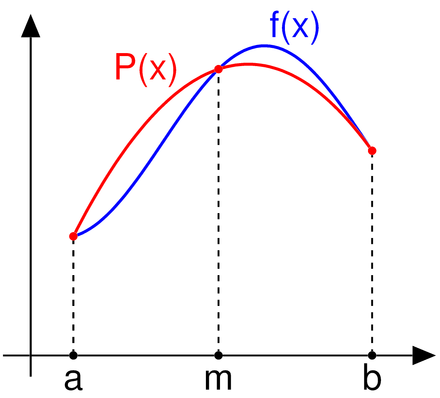
\includegraphics[scale=0.3]{sim_int.png}
\caption{Aproximation of Simposon's formula}
\end{wrapfigure}


 \begin{figure}[!h]
\centering
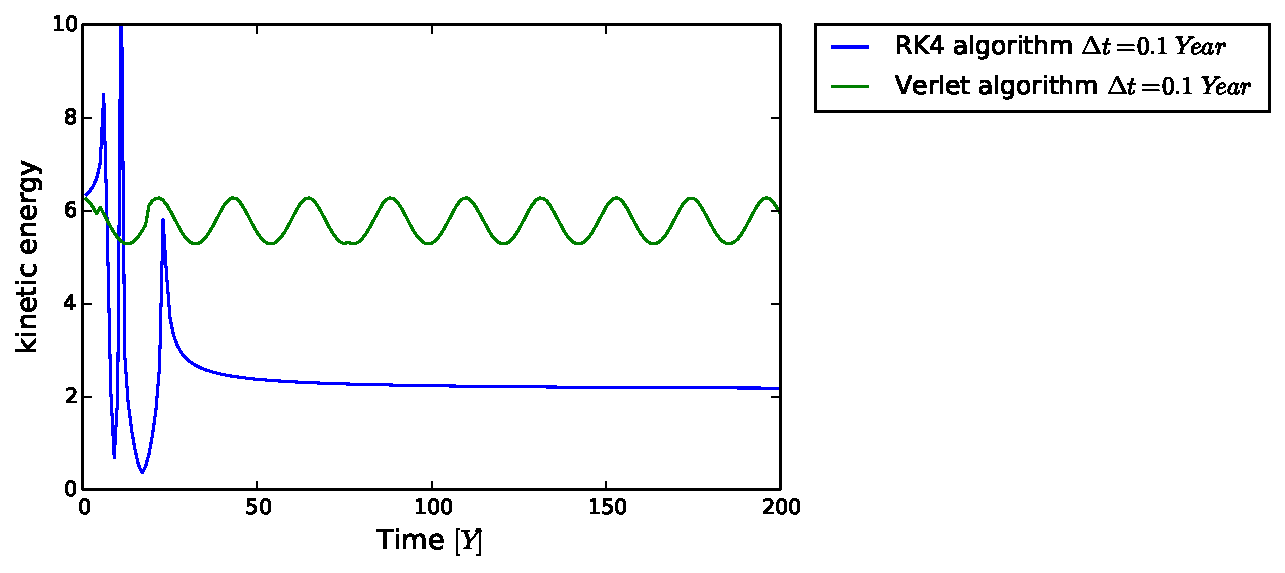
\includegraphics[width=1.02\textwidth]{outvel.pdf}
\caption{graf}
\end{figure}


A grapghic interpreation of the algorithm is very usefull to understan better it:

prova ciao !!ee 33
32
\section{Tuned Program}
\section{Energy states and probability functions}\label{2electrons}

\pagebreak
\section{Analytic Solution}
Prova hello!
\pagebreak
\section{Conculsions}

\section{References}
\begin{itemize}
\item M. Hjorth-Jensen, 
Computational Physics, University of Oslo (2013).
\item M. Hjorth-Jensen, 
Project3, University of Oslo (2013).
\item www.cplusplus.com
\end{itemize}



\end{document}
